\documentclass[12pt]{article}
\usepackage[magyar]{babel}
\usepackage{t1enc}
\usepackage{hulipsum}
\usepackage{tikz}
\usepackage{xcolor}

\begin{document}
\author{Nagy Balázs}
\title{11. gyakorlat}
\maketitle
\newpage

\section{Házikó}

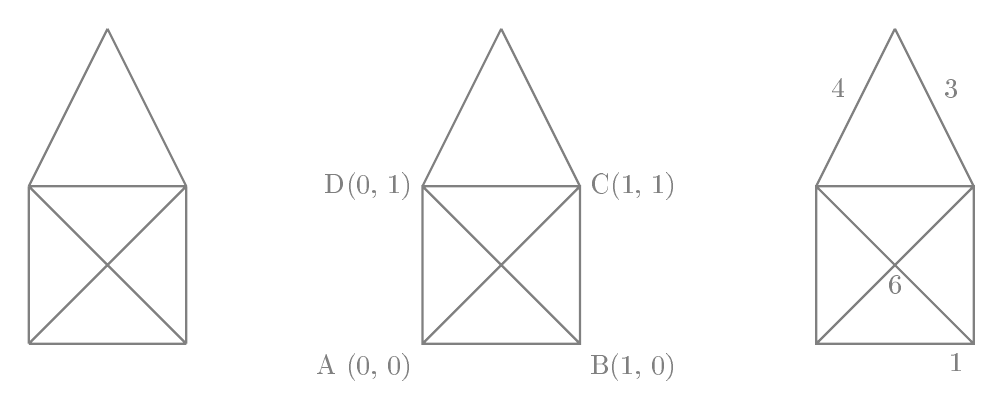
\begin{tikzpicture}
\draw[gray, thick] (0, 0) -- (2, 0) (0, -2) -- (2, -2) (0, 0) -- (0, -2)
(2, 0) -- (2, -2) (0, 0) -- (2, -2) (2, 0) -- (0, -2) (0, 0) -- (1, 2)
(2, 0) -- (1, 2);

\quad
\draw[gray, thick] (5, 0) rectangle (7, -2) (5, 0)node[left]{D(0, 1)} -- (7, -2)node[below right]{B(1, 0)} (7, 0) node[right]{C(1, 1)} -- (5, -2) node[below left]{A (0, 0)} (5, 0) -- (6, 2) (7, 0) -- (6, 2)
;

\quad
\draw[gray, thick] (10, 0) rectangle (12, -2)node[below left]{1} (10, 0)--(12, -2) (12, 0)--(10, -2)node[midway, below]{6} (10, 0)--(11, 2)node[midway, above left]{4} (12, 0)--(11, 2)node[midway, above right]{3};
\end{tikzpicture}


\section{Egységkör}

\begin{minipage}{0.7\textwidth}
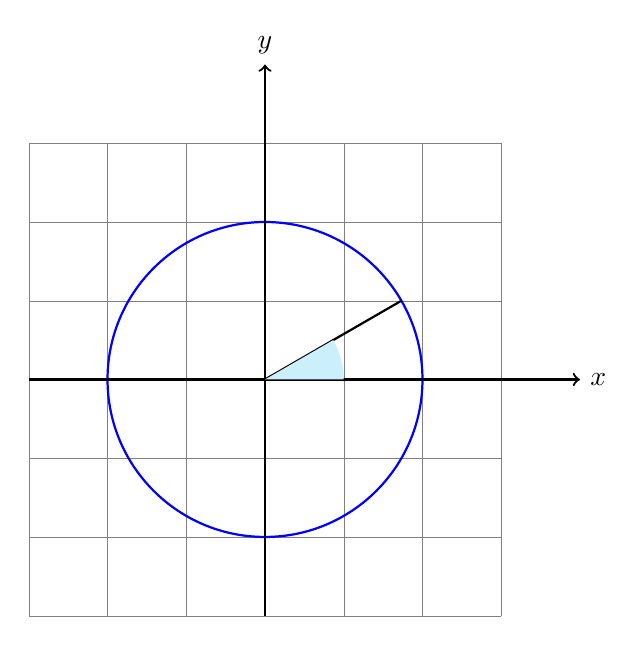
\begin{tikzpicture}[scale=2]

\draw[gray, thick, step=0.5, help lines, ultra thin](-1.5, -1.5) grid (1.5, 1.5);
\draw[blue, thick](0, 0) circle (1);
\draw[black, thick](0, 0);
\draw[->,thick] (-1.5,0)--(2,0) node[right]{$x$};
\draw[->,thick] (0,-1.5)--(0,2) node[above]{$y$};
\draw[black, thick] (0, 0) -- (30:1);
\fill[fill=cyan!20!white]
    (0,0) -- (0.5,0) arc (0:30:0.5);
    
\quad
asddaw

\end{tikzpicture}
\end{minipage}
\begin{minipage}{.7\textwidth}
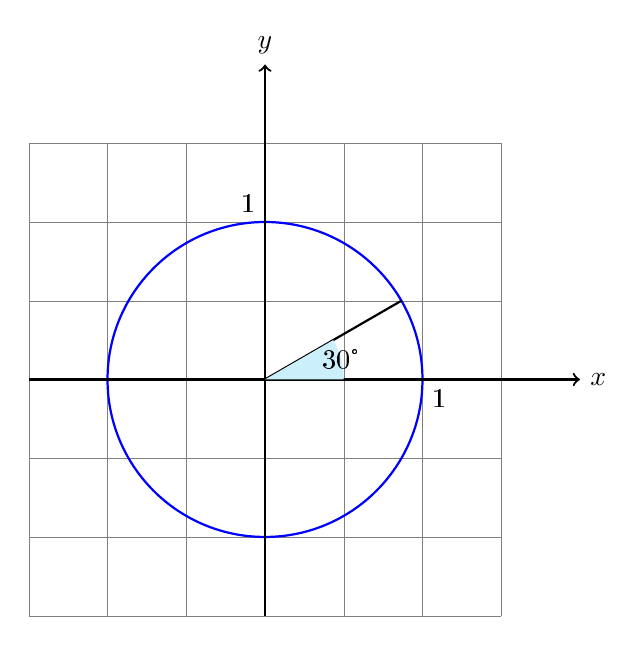
\begin{tikzpicture}[scale=2]
\draw[gray, thick, step=0.5, help lines, ultra thin](-1.5, -1.5) grid (1.5, 1.5);
\draw[blue, thick](0, 0) circle (1);
\draw[black, thick](0, 0);
\draw[->,thick] (-1.5,0)--(2,0) node[right]{$x$};
\draw[->,thick] (0,-1.5)--(0,2) node[above]{$y$};
\draw[black, thick] (0, 0) -- (30:1);
\fill[fill=cyan!20!white]
    (0,0) -- (0.5,0) arc (0:30:0.5)node[midway]{30°};
\draw (0, 1)node[above left]{1} (1, 0)node[below right]{1};
\end{tikzpicture}
\end{minipage}


\section{Kitöltések}
\tikz{ \shade[shading=radial, outer color=black, inner color=white] (0,0) -- ++(1,0) -- ++(60:1)
-- ++(120:1) -- ++(180:1) --++ (240:1)-- cycle ;

\shade[top color=blue, bottom color=green] (6,0) -- ++(1,0) -- ++(60:1)
-- ++(120:1) -- ++(180:1) --++ (240:1)-- cycle ;

\filldraw[fill=green, draw=red, fill opacity=0.5, opacity=0.3] (4, 0) rectangle (2, 2);

\filldraw[fill=yellow, draw=red, fill opacity=0.5, opacity=0.3] (5, 0) rectangle (3, 2);

\shade[shading=ball, ball color=gray]
(9,1) circle (1);

\draw (12, 0) -- ++(45:1) --++ (135:1) --++(225:1) -- cycle;}


\end{document}